% !TEX root = ../thesis-example.tex
%
\chapter{Metodologia}
\label{Metodologia}

En este capitulo se presenta el metodo y algoritmos desarrollados para calculo de la entropia en mercados financieros.
La metodologia presentada tiene como objetivo ayudar a detectar si un mercado es \textit{estable} en el tiempo a partir de la entropia calculada.
Adicionalmente, el metodo propuesto puede ser utilizado para detectar momentos (fechas) en los que la entropia es minima. 
Esto se traduce como un intervalo de tiempo en el que el precio no cambia significativamente.


\section{Algoritmo para el calculo de entropia simple}
\label{sec_algorithm}
La metodologia implementada para el calculo de la entropia asi como el procesamiento de datos se presenta en el diagrama \ref{diagramaentropia1}.


\begin{figure}[h]
	\centering
	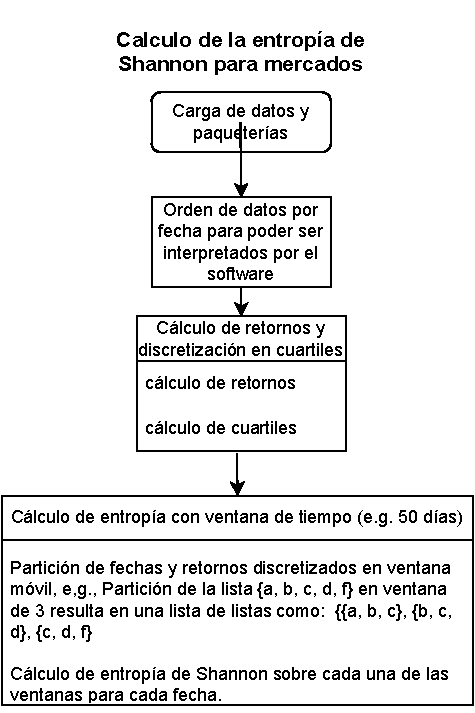
\includegraphics[width=0.7\linewidth]{figures/diagrama_entropia1}
	\caption{Diagrama del algoritmo utilizado para el c\'alculo de entrop\'ia de Shanon en mercados financieros.}
	\label{diagramaentropia1}
\end{figure}

En este diagrama se identifican cuatro etapas principales:

\begin{itemize}
	\item Carga de datos
	\item Pre-procesamiento de datos
	\item Calculo de retornos y cuartiles
	\item Calculo de entropia
\end{itemize}

Los algoritmos presentados en esta tesis fueron desarrollados en el lenguage de programacion Wolfram Mathematica y Matlab.


\subsection{Procesamiento de datos de precios de mercados}
\label{sec_data}
Los precios de los mercados utilizados en esta Tesis fueron obtenidos del portal Yahoo Finance. 
Cabe mencionar que los precios son registrados cada 24h excepto los dias sabado y domingo.
Se descargaron las datos de precios entre DD/MM/YYYY y DD/MM/YYYY de los mercados AAA, BBB, CCC, y DDD.

Un ejemplo de la base de datos de precios descargada se presenta en la tabla \ref{ejemplo_data}.
Las columnas de la base de datos corresponden a la fecha en la que se realizo el registro de precio respectivo.
Las bases de datos de cada uno de los mercados fueron depuradas y ordenadas. Esta depuracion corresponde a identificar y eliminar las fechas en las que no hay precio registrado. De este modo se evitan errores de calculo.

\begin{table}
\begin{center}
\begin{tabular}{|c|c|}
	\hline 
	Fecha & precio \\ 
	\hline 
	DD/MM/YYYY & $$$$ \\ 
	DD/MM/YYYY & $$$$ \\ 
	DD/MM/YYYY & $$$$ \\ 
	\hline 
\end{tabular} 
	\label{ejemplo_data}
	\caption{Ejemplo de base de datos de mercados financieros.}
\end{center}
\end{table}

\subsection{Calculo de retornos de precios de mercados}
\label{sec_retornos}
Luego que se han cargado los datos, y se han ordenado es necesario calcular los retornos de los precios. 
%y ello conlleva a que no va a haber una media central en los datos. 
Los retornos permiten analizar fácilmente la tasa de cambio en el tiempo.
En esta Tesis se eligio trabajar con los retornos de los precios y no con los precios directamente debido a las propiedades de los retornos presentadas en la subseccion \ref{retornos}.
Aunque los retornos son una mejor representación de los precios, aún presentan picos que sobresalen de la media. 
%La estandarización permite destacar los retornos que realmente son relevantes. 
%%%-----NO SE APLICO ESTANDARIZACION NO ?????
%Ya que cada retorno ha sido estandarizado con su respectiva fecha,  
Posteriormente se procede a discretizar los retornos mediante un proceso que divide en Q quantiles a los retornos.
Por ejemplo, la Tabla \ref{quantile_example} muestra un ejemplo de discretizacion de los retornos en cuatro cuartiles. 
En este ejemplo a cada cuartil se le asigna la etiqueta 1, 2, 3, 4 dependiendo del intervalo al que corresponde el valor de retorno.
De este modo, la Tabla \ref{ejemplo_data-returns} muestra un ejemplo de etiquetado para los retornos calculados sobre una base de datos.

\begin{table}	
\begin{center}
	\begin{tabular}{ |r | l | c| }
		\hline
		Cuartiles &  Valor de retorno & Etiqueta  \\ \hline
		Primer cuartil & $(-\infty , Q_2)$ & 1 \\
		Segundo cuartil & $[Q_2 , Q_3)$   & 2\\ 
		Tercer cuartil &  $[Q_3 , Q_4)$   & 3 \\
		Cuarto cuartil & $[Q_4 , \infty)$ &4\\ 
		\hline
	\end{tabular}
	\label{quantile_example}
		\caption{Intervalos de cuartiles y etiquetas aplicadas a los retornos.}
\end{center}
\end{table}


\begin{table}
	\begin{center}
	\begin{tabular}{|c|c|c|}
		\hline 
		Fecha & retorno & cuartil \\ 
		\hline 
		DD/MM/YYYY & $$$$ & 1\\ 
		DD/MM/YYYY & $$$$ & 2\\ 
		DD/MM/YYYY & $$$$ & 4\\ 
		\hline 
	\end{tabular} 
	\label{ejemplo_data-returns}
	\caption{Ejemplo de etiquetado para una base de datos de mercados financieros.}
\end{center}
\end{table}

\subsection{Calculo de la entropia}
\label{sec_entropia}
El calculo de la entropia se realizo de acuerdo a la ecuacion de Shannon \ref{entropySha}.
Para poder calcular la entropia se calculo la probabilidad de cada etiqueta sobre intervalos de tiempo glisantes de $\Delta t_{ent})$.
Los retornos y etiquetas fueron calculados y asignados como se explico en la seccion anterior. 
Con los intervalos dados por los cuartiles y la discretización de los retornos se obtiene todo lo necesario para calcular la entropía.
La ventana de tiempo glisante para el calculo de la entropía se corresponde a subconjuntos de datos agrupados en listas de N elementos.
En la Tabla \ref{entropytable} se muestra un ejemplo de la entropia calculada para un conjunto de datos. 
La ventana glisante aplicada para el calculo de entropia en este ejemplo es de 50 dias.

\begin{table}
	\begin{center}
	\begin{tabular}{|c|c|c|}
		\hline 
		Fecha & retorno & entropia \\ 
		\hline 
		DD/MM/YYYY & $$$$ & N entropia\\ 
		DD/MM/YYYY & $$$$ & N entropia\\ 
		DD/MM/YYYY & $$$$ & N entropia\\ 
		\hline 
	\end{tabular} 
	\label{entropytable}
	\caption{Ejemplo de entropia calculada para una base de datos de mercados financieros.}
\end{center}
\end{table}




\section{Calculo de entropía con retornos de medias moviles}
\label{metodo_MAV}
El metodo explicado en la Seccion anterior fue estudiado con una modificacion en el calculo de retornos.
Dicha modificacion consiste en el calculo de la media del precio sobre una ventana glisante de tiempo $\Delta t_{MAV})$(i.e., media movil) (ver Figura \ref{entropiamav}). 
El intervalo de la ventana glisante impacta directamente la curva de precios.
De este modo se observa que una ventana glisante grande (e.g. 50 dias) tiene un efecto de suavizado de la curva mas claro que una ventana corta (e.g., 10 dias) ver Figura \ref{ejemplo-medias moviles}. 

Una vez que las medias moviles de precio son calculadas, se calculan los retornos como dado por la Ecuacion \ref{retornos}.
Despues se aplica el metodo descrito en la Seccion \ref{sec_entropia} para calcular la entropia.
Las observaciones asi como conclusiones respecto a la aplicacion de medias moviles seran discutidas en profundidad en la seccion \ref{Conclusiones}.


\begin{figure}
	\centering
	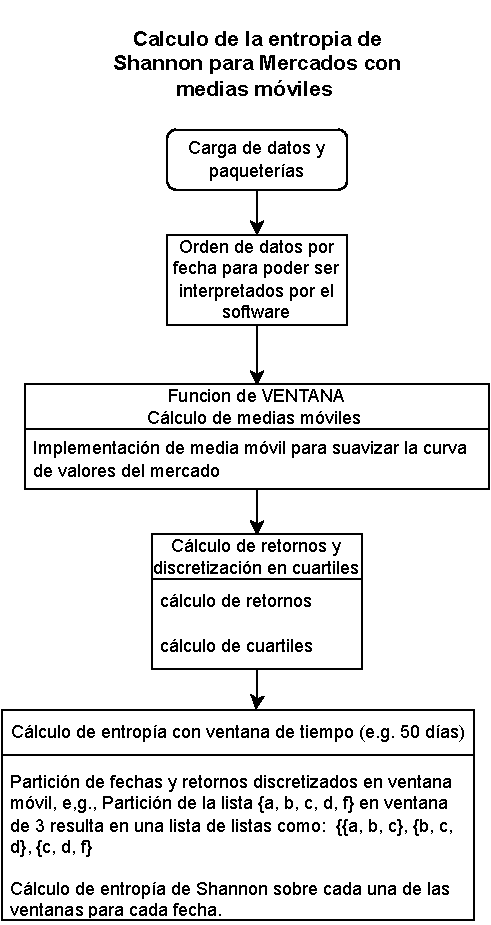
\includegraphics[width=0.7\linewidth]{figures/entropiaMAV}
	\caption{Diagrama del algoritmo utilizado para el c\'alculo de entrop\'ia de Shanon en mercados financieros con medias m\'oviles.}
	\label{entropiamav}
\end{figure}



\section{Simulacion de un mercado eficiente}

Para fines de comparacion y validacion de la metodologia propuesta en las Secciones previas a mercados financieros reales se realizo una simulación de un mercado eficiente.
Esta simulacion utiliza los datos del mercado real para calcular la media y desviación estándar  de los retornos (no estandarizados) de los precios reales. 
Posteriormente se obtienen retornos simulados a los cuales se les asigna una fecha.

A partir de este punto se realizaron dos simulaciones que se pueden apreciar en el diagrama \ref{simulacion}.
La primera es que a dichos retornos simulados se les aplica el proceso para el cálculo de entropía de la figura \ref{diagramaentropia1}.
En la segunda se aplica el proceso de medias móviles como se presenta en \ref{entropiamav}.

\begin{figure}
	\centering
	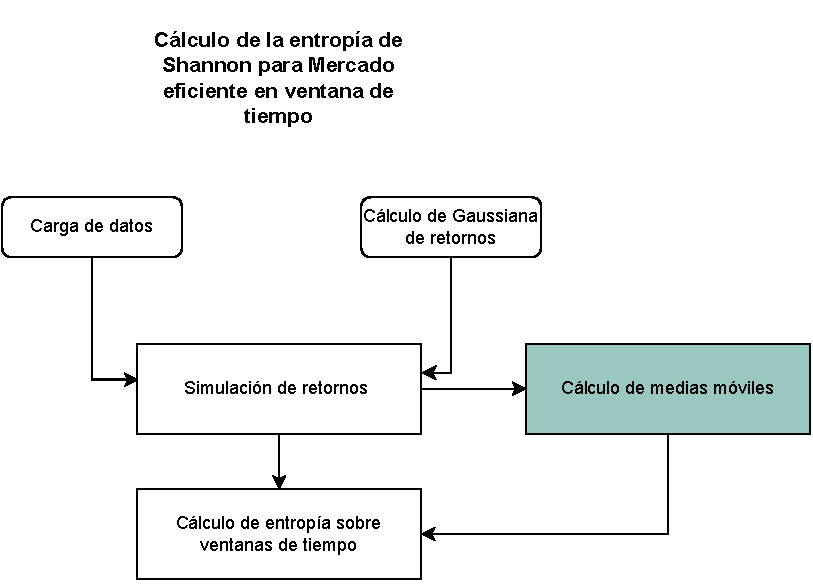
\includegraphics[width=0.9\linewidth]{figures/simulacion}
	\caption{Diagrama del algoritmo de calculo de entropia para la simulacion de mercado eficiente. }
	\label{simulacion}
\end{figure}

La simulacion de mercado eficiente nos proporciona puede ser utilizada para calcular un umbral que permita seleccionar los valores de entropía mínima en los mercados reales. 
 
\section{Ajuste de distribuciones estadisticas}

Para poder seleccionar los valores de minima entropia se aplico un ajuste de distribuciones estadisticas a los valores de entropia.
Este ajuste es realizado utilizando el paquete \textit{Distribution Fitter} de Matlab.
Este paquete esta compuesto de una aplicacion que permite de ajustar de manera interactiva funciones de probabilidad.
Las funciones de ajuste pueden tambien ser utlizadas fuera del ambiente interactivo.

Las distribuciones que seran ajustadas son:

\begin{itemize}
	\item tt
	\item toto
\end{itemize}



\section{Busqueda de minimos de entropia}

Uno de los objetivos de esta Tesis es buscar un metodo que permita la identificacion de minimos de entropia en los mercados financieros.
Sin embargo, en la metodologia descrita en la Seccion \ref{metodo_MAV} se observa que existen tres parametros dados por el usuario:
\begin{itemize}
	\item la talla de ventana glisante $\Delta t_{MAV})$ para suavizado de la curva de precios,
	\item la talla de ventana glisante $\Delta t_{ent})$ para el calculo de la entropia y
	\item el numero de cuantiles $Q$ sobre los cuales se calcula la entropia de Shannon.
\end{itemize}

Estos parametros actuan directamente sobre el calculo de la entropia de la siguiente manera: 
el valor de $\Delta t_{MAV})$ tiene un impacto directo sobre el suvizado de la curva de precios, y como consecuencia, sobre la determinacion de los valores de entropia. 
$\Delta t_{ent})$ tiene un impacto en el numero de muestras utilizadas en el calculo de la entropia, este valor impacta directamente el valor de la probabilidad de los valores de $Q$. 
Por otro lado, el valor de $Q$ es el numero de categorias utilizadas para el calculo de la entropia. 
Un valor muy grande de $Q$ puede diluir los minimos de entropia mientras que un valor muy pequeno puede resultar en una perdida de la informacion.

Para mejorar el calculo de la entropia se realizo una evaluacion de los valores de $\Delta t_{MAV})$, $\Delta t_{ent})$ y $Q$.
Esta evaluacion busca maximizar el numero de minimas entropias detectadas.


	

